\documentclass[a4paper,12pt]{article}
\usepackage{mathtools}
\usepackage{graphicx,url}
\usepackage[english]{babel}

\graphicspath{{.}{images/}}
\pdfimageresolution=600

\begin{document}

\title{QMClique: A Proposal and Questions for Quantum Maximal Clique Algorithm}
\author{Gustavo C. G. van Erven\footnote{gustavo.erven@cgu.gov.br}}
\maketitle

\begin{abstract}
	Finding cliques in graphs is well know computing problem. These notes present an algorithm for maximal cliques and a research question for its implementation in a quantum computer. 
\end{abstract}

\section{Definitions}

A Graph $G(V,E)$ is a set of vertices $V = \{v_1,v_2,\dots,v_n\}$ with set $E$ of relations between them, $E = \{e_1,e_2,\dots,e_m\}$ and $e_i = (u,v) | u,v \in V$.

A Clique is a subgraph of $G(V,E)$, which all vertices are connected to each other.

Theorem: Let $W_i$ be the set of all adjacent vertices for vertex $i$, union with $i$, $W_i = V_{adj(i)} \cup \{v_i\}$, if C is a maximal clique of size k:
\begin{equation}\label{eq:clique}
C = \{\{v_i\} \cup \{v_{i+1}\} \cup \dots \cup \{v_k\}\} = \{W_i \cap W_{i+1} \cap \dots \cap W_{k}\}
\end{equation}

The right side of Equation~\ref{eq:clique} has all vertices in the clique $C$. Therefore, they must be present in the left side, because all vertex in a clique are connected each other. The intersection have only clique's vertex, because they are the elements in commune between all of them. If a some vertex is in the left side and not in the union, the vertex will be a common vertex, and the right side is not complete. 

If there is a vertex in the union that are not in the maximal clique, it will not be present in the intersection, because it will not be connected to all set's elements.

\section{Checking a maximal clique}

Let $H_i = V_{adj(i)} \cup \{v_i\}$, we can represent it as a vector, such as shown in Equation~\ref{eq:vech}, where $e_i$ is equal to 1 if the vertex i is connected to the node in the index position.

\begin{equation}\label{eq:vech}
W_i = 
	\begin{bmatrix}
		e_{1} \\
		e_{2} \\
		\vdots  \\
		e_{n}
	\end{bmatrix}
\end{equation}

Therefore, the set with all vectors $H_i$ is equivalent to the adjacent matrix in below.

\begin{equation}
W = 
	\begin{bmatrix}
	1 & e_{1,2} & \cdots & e_{1,n} \\
	e_{2,1} & 1 & \cdots & e_{2,n} \\
	\vdots  & \vdots  & \ddots & \vdots  \\
	e_{n,1} & e_{n,2} & \cdots & 1 
	\end{bmatrix}
\end{equation}

Let $A$ be a vector represents the presence of the vertex $v_i$ when $a_i$ is set to 1 or 0 otherwise, such that:

\begin{equation}
A = 
\begin{bmatrix}
a_{1} \\
a_{2} \\
\vdots  \\
a_{n}
\end{bmatrix}
\end{equation}

And $A_i$ a vector composed by n elements $a_i \in A$:

\begin{equation}
A_i = 
\begin{bmatrix}
a_{i} \\
a_{i} \\
\vdots  \\
a_{i}
\end{bmatrix}
\end{equation}

According with Equation~\ref{eq:clique}, if a vector $A$ is given, we can check if it is a maximal clique verifying if the intersection of vectors $W_i$ are equal to $A$. The intersection can be calculated with AND ports.

\begin{equation}
	\text{A is a maximal clique iff is equal to } W_i \land W_{i+1} \land \dots \land W_k
\end{equation}

Now, we can compute a true value which represents if the input vector $A$ is a maximal clique. At first, if $a_i$ is present, the vector $W_i$ must be used. Otherwise, the presence of the vertex must be ignores. We can ignore the vector change all the values to 1, then it will not influence the AND operations. The Equation~\ref{ex:removea1} shows an example for a $W_i$ vector. 

\begin{align}
	\neg A_i \lor (A_i \land W_i) \\
	(\neg A_i \lor A_i) \land (\neg A_i \lor W_i) \\
	\neg A_i \lor W_i \label{ex:removea1}
\end{align}

Therefore, if $a_1$ is 0, all the values in $W_i$ will be changed to 1, and it will not affect the AND operations. Now we can generalize to check a input $A$ over all vectors in $W$. Let $O$ be the output vector for the AND operations, thus:

\begin{equation}
	O = (\neg A_1 \lor W_1) \land (\neg A_2 \lor W_2) \land \dots \land (\neg A_n \lor W_n)
\end{equation}

Therefore, $O_i$ is the result for element $a_i$, where $w_{ij}$ is the element $j$ for the vector $W_i$:

\begin{equation}
O_i = (\neg a_1 \lor w_{11} \land (\neg a_2 \lor w_{21}) \land \dots \land (\neg a_n \lor w_{n1})
\end{equation}

Now, $A$ will be a clique if the output $O$ is equal to $A$. We can summarize it through a single value. Let $R$ be a boolean variable, such that:

\begin{align}
	U = (O \oplus \neg A)\\
	R = u_1 \land u_2 \land \dots \land u_n\\
	R = (o_1 \oplus \neg a_1) \land (o_2 \oplus \neg a_2) \land \dots \land (o_n \oplus \neg a_n)
\end{align}

Therefore, if $R$ is true, the vector input $A$ is a maximal Clique. Note that, if $A$ is a subset of maximal Clique, $R$ will be false because all vertices with $a_i = 0$ will have their values changes to 1. Therefore, if some node $i$ is not present, but is adjacent to the selected vertices in $A$, the output value will be true for $O_i$, and the final verification will return false, such that the $O_i = 1$ and $a_i = 0$.

If the algorithm is implement in a program, the time complexity will be $O(n^2)$, since we need $n$ operation by each $n$ vertex to generate the $O$ vector, and more $n$ operations to calculate $R$.

\section{Using Quantum ports}

The algorithm can be implemented in a quantum computer using the Toffoli gate. The Equation~\ref{ex:removea1} can be modified to make the implementation easier, as shown in Equation~\ref{ex:remtof}.

\begin{equation}
	\neg A_i \lor W_i = 1 \oplus A_i W_i \label{ex:remtof}
\end{equation}

The AND port can be implemented with a Toffoli gate as present in Equation~\ref{ex:andtof} 

\begin{equation}
	A \land B = 0 \oplus AB \label{ex:andtof}
\end{equation}

These gates can replace the boolean operations in the maximal clique algorithm. A Hadamard gate can be used in the input vector $A$ to create a superposition with all possible values.

The Figure~\ref{fig:qcircuit} presents an implementation for a two vertices graph without edges.

\begin{figure}[!ht]
	\label{fig:qcircuit}
	\centering
	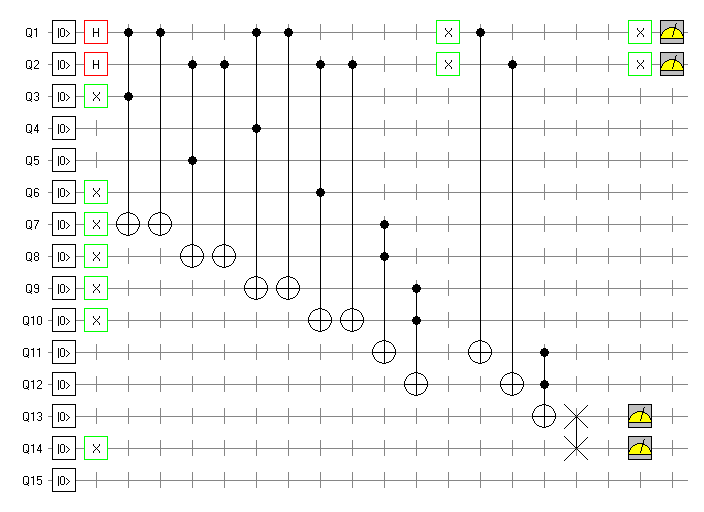
\includegraphics[width=1\textwidth]{qclique}
	\caption{Quantum circuit for two vertices graph.}
\end{figure}

The $W$ matrix for this example is $\bigl(\begin{smallmatrix}
1&0 \\ 0&1 \end{smallmatrix} \bigr)$ and must be true only for $\bigl(\begin{smallmatrix} 1\\0 \end{smallmatrix} \bigr)$ and $\bigl(\begin{smallmatrix} 0\\1 \end{smallmatrix} \bigr)$ inputs.

Note that will be necessary $n$ qubits for $A$, $n^2$ qubits for $W$, $n^2$ qubits to keep the $(1 \oplus A_i W_i)$ operations, $n$ qubits for the $O$ vectors and one to the result $R$.

\section{Conclusions and Question}

The algorithm to verify a maximal clique can be implemented in a quantum computer using Toffoli gates. The Hadamard gate can be used to create a superposition in the input vector $A$. However, we are only interested in values that makes $R$ true, which implies that in a maximal clique. \textbf{The question is: is there an entangle state that we can use to force the result $R$ be true and makes $A$ to collapse to a maximal clique? Could the swap gate X do this? And if it exists, is there a way to take only the maximum cliques superpositions?}

\end{document}